%%%%%%%%%%%%%%%%%%%%%%%%%%%%%%%%%%%%%%%%%
% Short Sectioned Assignment
% LaTeX Template
% Version 1.0 (5/5/12)
%
% This template has been downloaded from:
% http://www.LaTeXTemplates.com
%
% Original author:
% Frits Wenneker (http://www.howtotex.com)
%
% License:
% CC BY-NC-SA 3.0 (http://creativecommons.org/licenses/by-nc-sa/3.0/)
%
%%%%%%%%%%%%%%%%%%%%%%%%%%%%%%%%%%%%%%%%%

%----------------------------------------------------------------------------------------
%	PACKAGES AND OTHER DOCUMENT CONFIGURATIONS
%----------------------------------------------------------------------------------------

\documentclass[paper=letter, fontsize=11pt]{scrartcl} % A4 paper and 11pt font size

\usepackage[margin=1.0in]{geometry}

\usepackage[T1]{fontenc} % Use 8-bit encoding that has 256 glyphs
%\usepackage{fourier} % Use the Adobe Utopia font for the document - comment this line to return to the LaTeX default
\usepackage[english]{babel} % English language/hyphenation
\usepackage{amsmath,amsfonts,amsthm} % Math packages

\usepackage{sectsty} % Allows customizing section commands
%\allsectionsfont{\centering\normalfont\scshape} % Make all sections centered, the default font and small caps
%\allsectionsfont{\scshape} % Make all sections centered, the default font and small caps

\usepackage{fancyhdr} % Custom headers and footers
\pagestyle{fancyplain} % Makes all pages in the document conform to the custom headers and footers
\fancyhead{} % No page header - if you want one, create it in the same way as the footers below
\fancyfoot[L]{} % Empty left footer
\fancyfoot[C]{} % Empty center footer
\fancyfoot[R]{\thepage} % Page numbering for right footer
\renewcommand{\headrulewidth}{0pt} % Remove header underlines
\renewcommand{\footrulewidth}{0pt} % Remove footer underlines
\setlength{\headheight}{13.6pt} % Customize the height of the header

\numberwithin{equation}{section} % Number equations within sections (i.e. 1.1, 1.2, 2.1, 2.2 instead of 1, 2, 3, 4)
\numberwithin{figure}{section} % Number figures within sections (i.e. 1.1, 1.2, 2.1, 2.2 instead of 1, 2, 3, 4)
\numberwithin{table}{section} % Number tables within sections (i.e. 1.1, 1.2, 2.1, 2.2 instead of 1, 2, 3, 4)

%\setlength\parindent{0pt} % Removes all indentation from paragraphs - comment this line for an assignment with lots of text

% For code blocks.
\usepackage{listings}

% For figures.
\usepackage{graphicx}
\usepackage{subcaption}

% For subsection formatting.
\renewcommand{\thesubsection}{(\alph{subsection})}

\usepackage{titlesec}
%\titleformat{\subsection}[runin]{\normalfont\large}{\thesubsection}{1em}{}

%----------------------------------------------------------------------------------------
%	TITLE SECTION
%----------------------------------------------------------------------------------------

\newcommand{\horrule}[1]{\rule{\linewidth}{#1}} % Create horizontal rule command with 1 argument of height

\title{
\normalfont \normalsize
%\textsc{university, school or department name} \\ [25pt] % Your university, school and/or department name(s)
\horrule{0.5pt} \\[0.4cm] % Thin top horizontal rule
\huge MIT 16.31 - Project Report \\ % The assignment title
\horrule{2pt} \\[0.5cm] % Thick bottom horizontal rule
}

\author{W. Nicholas Greene} % Your name

\date{\normalsize2014.12.05} % Today's date or a custom date

\begin{document}

\maketitle % Print the title

%----------------------------------------------------------------------------------------
% Introduction
%----------------------------------------------------------------------------------------

\begin{figure}[h]
  \centering
  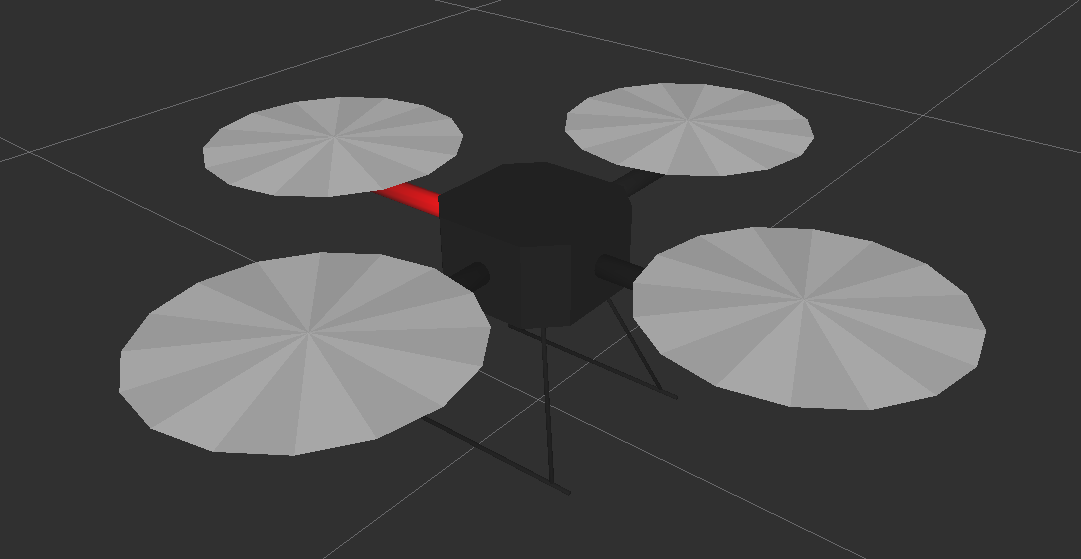
\includegraphics[width=0.75\textwidth]{quadrotor_screenshot_cropped}
  \caption{Simulated quadrotor using \texttt{hector\_quadrotor} \cite{2012simpar_meyer}.}
\end{figure}

\section{Introduction}
Autonomous navigation and control of micro-aerial vehicles (MAVs) is an increasingly popular
subject of academic research, with several key advances occurring over the last ten years.
Small, four-rotor craft (\textit{quadrotors}) are desirable platforms for this kind of
robotics research due to their ability to carry large sensor payloads and maintain stability
in the hover regime. There is significant interest, however, in having these types of vehicles
execute aggressive trajectories far from the hover state (e.g. flying quickly through
cluttered environments such as buildings and forests).

This project focuses on the implementation of a modern, nonlinear controller for stabilizing the
3D position and yaw angle of a quadrotor far from the hover regime based on \cite{lee2010geometric}.
A modified version of this controller was implemented in Python and validated
in simulation using the \texttt{hector\_quadrotor} simulator - a software package that simulates the
dynamics of a quadrotor using the Robot Operating System (ROS) and the Gazebo robot
simulation toolkit \cite{2012simpar_meyer, quigley2009ros, koenig2004design}. Results
show that the controller is able to successfully track aggressive trajectories with
significant linear and angular accelerations.


%----------------------------------------------------------------------------------------
% Geometric Control on SE3
%----------------------------------------------------------------------------------------
\section{Geometric Control on SE(3)}
Controlling a quadrotor's six degrees of freedom (3D position and 3D orientation) is a
non-trivial task for several reasons. First, the dynamics involved are non-linear, which
makes linear control schemes  such as proportional-integral-derivative (PID) controllers or
linear quadratic regulators (LQR) less attractive. Second, the quadrotor system state
does not lie in Euclidean space, but on the special Euclidean group SE(3) - the manifold composed
of 3D positions and 3D orientations ($\textrm{SE}(3) = \{\mathbb{R}^3 \times \textrm{SO}(3)\}$
where SO(3) is the special orthogonal group representing 3D rotations).
Finally, the system can only be controlled via the forces and torques produced by its
four rotors. (While this arrangement is beneficial from a modelling complexity standpoint,
it requires the interactions of all the rotors to effectively control the vehicle).

\subsection{Dynamics Model}
The equations governing the quadrotor's dynamics follow directly from Newton's second law
of motion:
\begin{align}
\dot{x} &= v \\
m \dot{v} &= m g e_3 - f R e_3 \\
\dot{R} &= R \hat{\Omega} \\
M &= J \dot{\Omega} + \Omega \times J\Omega
\end{align}
where $x \in \mathbb{R}^3$ and $v \in \mathbb{R}^3$ are the system's position and velocity,
$R \in \textrm{SO}(3)$ and $\Omega \in \mathbb{R}^3$
are the orientation (represented as a rotation matrix) and angular velocity (in the
body frame), $m \in \mathbb{R}$ and $J \in \mathbb{R}^{3 \times 3}$ are the mass
and intertia matrix (in the body frame), $f \in \mathbb{R}$ and $M \in \mathbb{R}^3$ are the
total thrust and torque from the rotors, $g \in \mathbb{R}$
is the gravitational acceleration constant, $e_3 \in \mathbb{R}^3$ is the downward pointing unit vector
in the standard (Right-Foward-Down) basis, and $\hat{\cdot}: \mathbb{R}^3 \rightarrow \textrm{so}(3)$
is the \textit{hat} operator, which maps vectors in $\mathbb{R}^3$ to the set of $3 \times 3$
skew-symmetric matrices (i.e. the Lie algebra so(3) associated with SO(3)).

The total thrust $f$ and torque $M = \begin{bmatrix} M_1 & M_2 & M_3\end{bmatrix}^T$
are related to the thrust from each motor $f_i$ by a linear transform:
\begin{align}
  \begin{bmatrix}
    f \\
    M_1 \\
    M_2 \\
    M_3
  \end{bmatrix}
  &=
  \begin{bmatrix}
    1 & 1 & 1 & 1\\
    0 & -d & 0 & d \\
    d & 0 & -d & 0 \\
    -c_{\tau f} & c_{\tau f} & -c_{\tau f} & c_{\tau f}
  \end{bmatrix}
  \begin{bmatrix}
    f_1 \\
    f_2 \\
    f_3 \\
    f_4
  \end{bmatrix}
\end{align}
where $d > 0$ is the length from the vehicle's center of mass to the rotors and
$c_{\tau f} > 0$ is a constant.

Given these parameters, the matrix above is invertible and the net thrust $f$ and
torque $M$ can be computed directly from the individual motor thrusts $f_i$.
The control scheme in \cite{lee2010geometric} therefore considers these two
quantities as the system's control inputs. Furthermore, the state of the system is considered
to be the tuple $(x, v, R, \Omega)$ and is assumed to be directly observed.

\subsection{Tracking Controller}
The approach in \cite{lee2010geometric} relates errors in the state space to the
control inputs needed to track a smooth trajectory $x_d(t) \in \mathbb{R}^3$ with
a desired heading direction or yaw angle, which is parameterized by the unit forward-facing
vector $f_d(t) \in \mathbb{R}^3$.

Note that the quadrotor cannot control its
position and orientation independently (it must pitch or roll to translate) and
therefore two of the three degrees of freedom related to orientation are constrained
by tracking the desired trajectory. The remaining degree of orientation freedom
(the yaw angle) is then chosen to most closely match the projection of the
desired forward vector $f_d(t)$ onto the horizontal plan defined by the quadrotor
body, resulting in the goal orientation $R_d$.

Finally, the control inputs $f$ and $m$ are determined by the following relations:
\begin{align}
  f &= -(-k_x e_x - k_v e_v -m g e_3 + m \ddot{x}_d) \cdot Re_3 \\
  M &= -k_R e_R - k_{\Omega} e_{\Omega} + \Omega \times J \Omega
       - J(\hat{\Omega}R^TR_d \Omega_d - R^TR_d \dot{\Omega}_d)
\end{align}
where $k_x$, $k_v$, $k_R$, and $k_{\Omega}$ are positive constants and
$e_x$, $e_v$, $e_R$, and $e_{\Omega}$ are tracking errors defined by
\begin{align}
  e_x &= x - x_d \\
  e_v &= v - v_d \\
  e_R &= \frac{1}{2}(R_d^TR - R^TR_d)^{\vee} \\
  e_{\Omega} &= \Omega - R^TR_d \Omega_d.
\end{align}
Note that $e_R$ and $e_{\Omega}$ are carefully formed to obey the topology of
SO(3) and that the \textit{vee}-map $\cdot^{\vee}: \textrm{so}(3) \rightarrow \mathbb{R}^3$ is the
inverse of the hat-map.

%% TODO: Info on errors and projection stuff?

%----------------------------------------------------------------------------------------
% Implementation
%----------------------------------------------------------------------------------------
\section{Implementation}
A modified version of the above controller was implemented in Python and validated
in simulation using the \texttt{hector\_quadrotor} package \cite{2012simpar_meyer}
and ROS Indigo \cite{quigley2009ros}.
Unfortunately, however, the package does not easily support controlling the quadrotor's total
thrust $f$ and torque $M$ (only the motor voltages can be directly set), so
the approach in \cite{lee2010geometric} was adapted
to take advantage of an existing PID controller available in the
stack that tracks linear and angular velocity.

This simple controller was considered to be an inner loop
of the system, resulting in new control inputs $v$ and $\Omega$. Using the
error forms described above, a new controller was devised:
\begin{align}
  v &= -k_x e - k_v e_v + v_d \\
  \Omega &= -k_R e_R - k_{\Omega} e_{\Omega} + \Omega_d.
\end{align}

Note that the form of $\Omega$ is not entirely correct as it does not obey the
topology of SO(3). Furthermore, the low-level PID controllers rely on Euler angles
and may therefore limit the full capabilities of the approach described in
\cite{lee2010geometric}. Nevertheless, this scheme proved sufficient for
executing complex trajectories in simulation using $k_x = 4m$, $k_v = 2.5m$,
$k_R = 15$, and $k_{\Omega} = 20$.

%----------------------------------------------------------------------------------------
% Results
%----------------------------------------------------------------------------------------
\pagebreak
\section{Results}
The modified controller was tested on two simulated trajectories: a simple circular
path (see Figure \ref{fig:circle_trajectory}) and a more complex path based on a
Lissajous curve (see Figure \ref{fig:lissajous_trajectory}).

\begin{figure}[h]
  \centering
  \begin{subfigure}[b]{0.5\textwidth}
    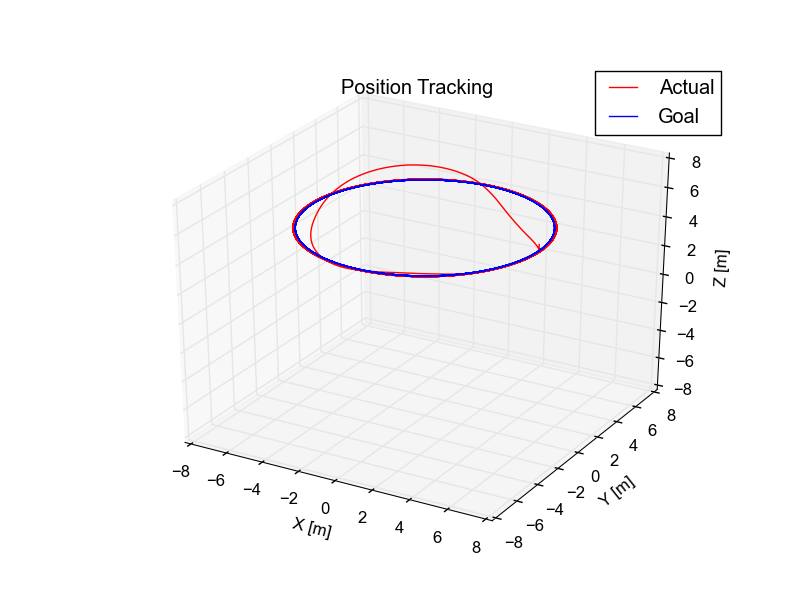
\includegraphics[width=\textwidth]{circle_trajectory}
    \caption{Circular trajectory}
    \label{fig:circle_trajectory}
  \end{subfigure}%
  ~ %add desired spacing between images, e. g. ~, \quad, \qquad, \hfill etc.
    %(or a blank line to force the subfigure onto a new line)
  \begin{subfigure}[b]{0.5\textwidth}
    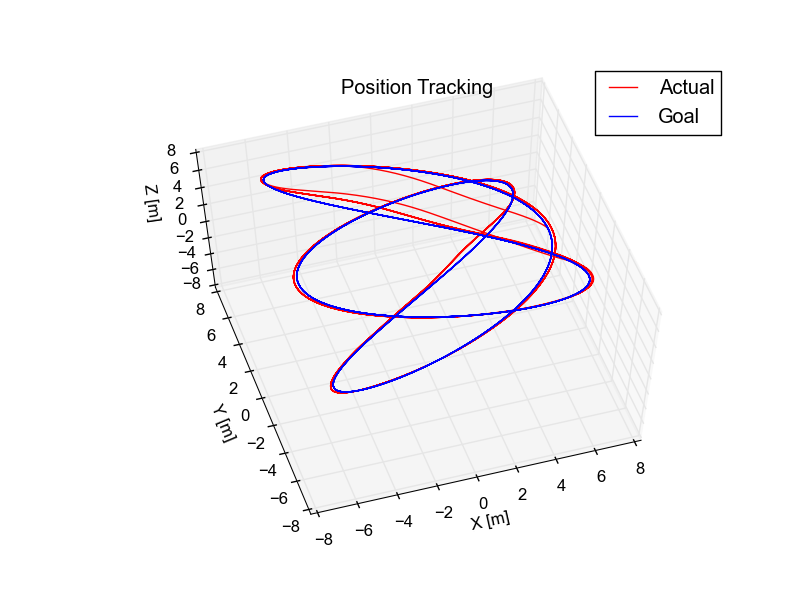
\includegraphics[width=\textwidth]{lissajous_trajectory}
    \caption{Lissajous trajectory}
    \label{fig:lissajous_trajectory}
  \end{subfigure}
  \caption{Desired trajectories (blue) with actual position (red).}
  \label{fig:trajectories}
\end{figure}

\subsection{Circle Trajectory}
The circular trajectory was defined by the following smooth parametric function:
\begin{align}
  x_d(t) &=
  \begin{bmatrix}
    R \cos(\omega t) \\
    R \sin(\omega t) \\
    Z
  \end{bmatrix}
\end{align}
where the radius of the curve $R = 6$ m, the height of the curve $Z = 5$ m,
and the period $T = 2 \pi / \omega = 9$ seconds.

The forward vector was set to $f_d(t) = \frac{v_d(t)}{||v_d(t)||}$, where the
velocity vector $v_d(t) = \dot{x}(t)$ is given by
\begin{align}
  v_d(t) &=
  \begin{bmatrix}
    -R \omega \sin(\omega t) \\
    R \omega \cos(\omega t) \\
    0
  \end{bmatrix}.
\end{align}

Figure \ref{fig:circle_performance} shows the tracking performance
of the controller. As one can see, the controller successfully tracks the circular
path, with steady state errors under 10 cm  (although some overshoot is present initially).
The RMSE for each component is shown in Table \ref{table:metrics}. Note that the
error in the $y$ direction is dominated by the initial overshoot (the steady state
error is less than 10 cm). The error for the forward direction was defined
to be the angular distance between the desired forward vector (projected onto the
horizontal body plane) and the actual forward vector and is less than 1.5 degrees.

\begin{figure}[h]
  \centering
  \begin{subfigure}[b]{0.45\textwidth}
    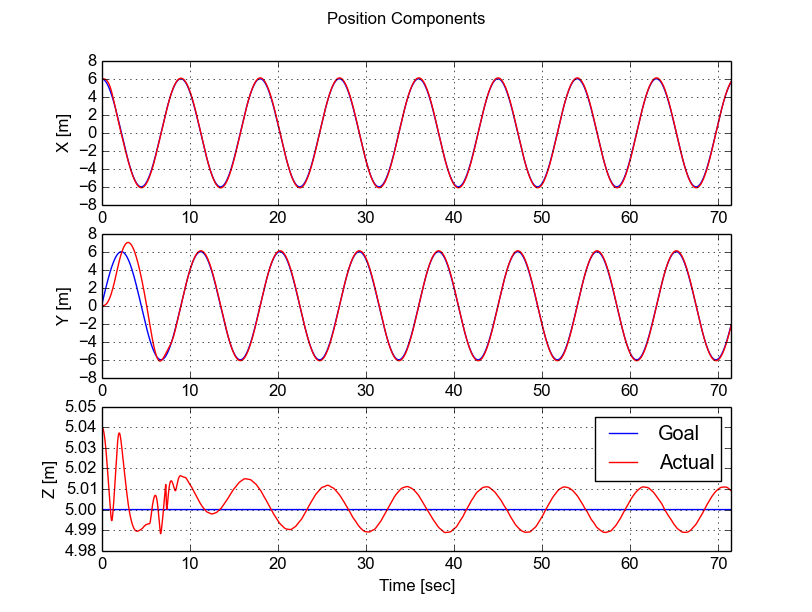
\includegraphics[width=\textwidth]{circle_position}
    \caption{Position}
    \label{fig:circle_position}
  \end{subfigure}%
  ~ %add desired spacing between images, e. g. ~, \quad, \qquad, \hfill etc.
    %(or a blank line to force the subfigure onto a new line)
  \begin{subfigure}[b]{0.45\textwidth}
    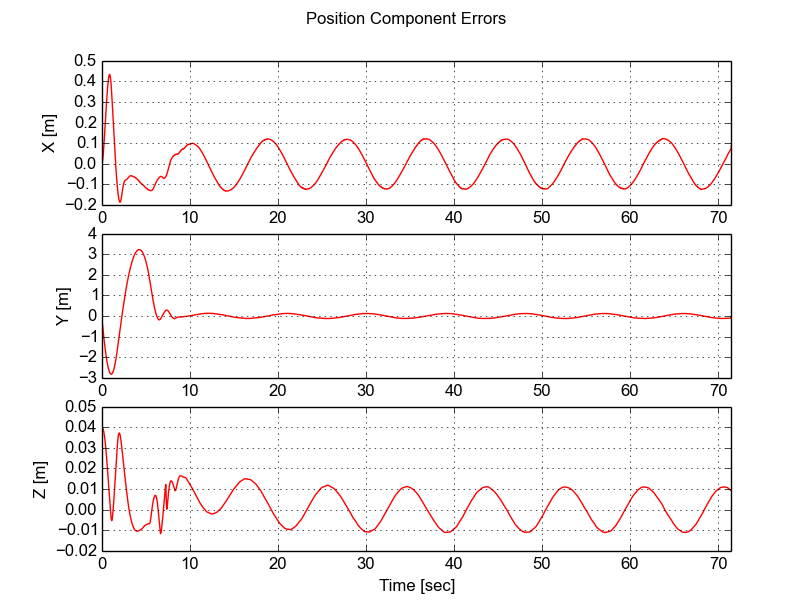
\includegraphics[width=\textwidth]{circle_position_errors}
    \caption{Position errors}
    \label{fig:circle_position_errors}
  \end{subfigure}

  \begin{subfigure}[b]{0.45\textwidth}
    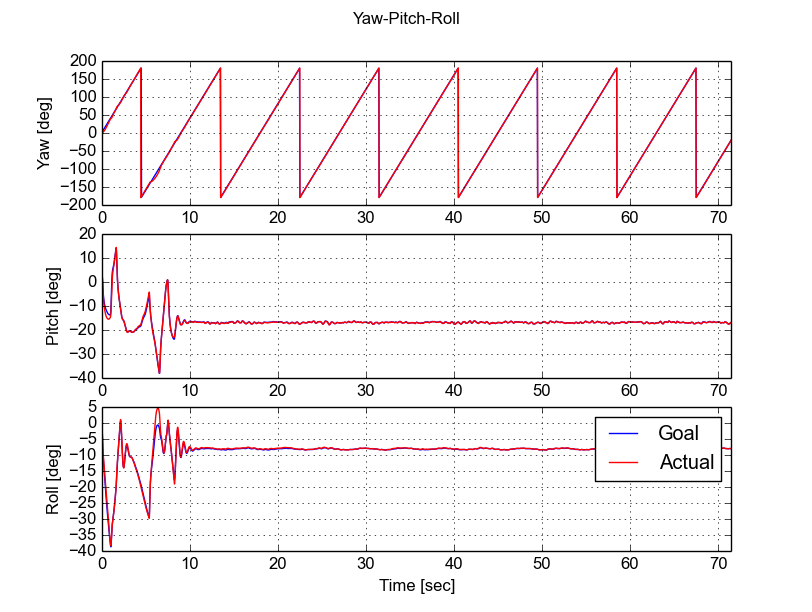
\includegraphics[width=\textwidth]{circle_yaw_pitch_roll}
    \caption{Yaw, pitch, and roll}
    \label{fig:circle_yaw_pitch_roll}
  \end{subfigure}%
  ~ %add desired spacing between images, e. g. ~, \quad, \qquad, \hfill etc.
    %(or a blank line to force the subfigure onto a new line)
  \begin{subfigure}[b]{0.45\textwidth}
    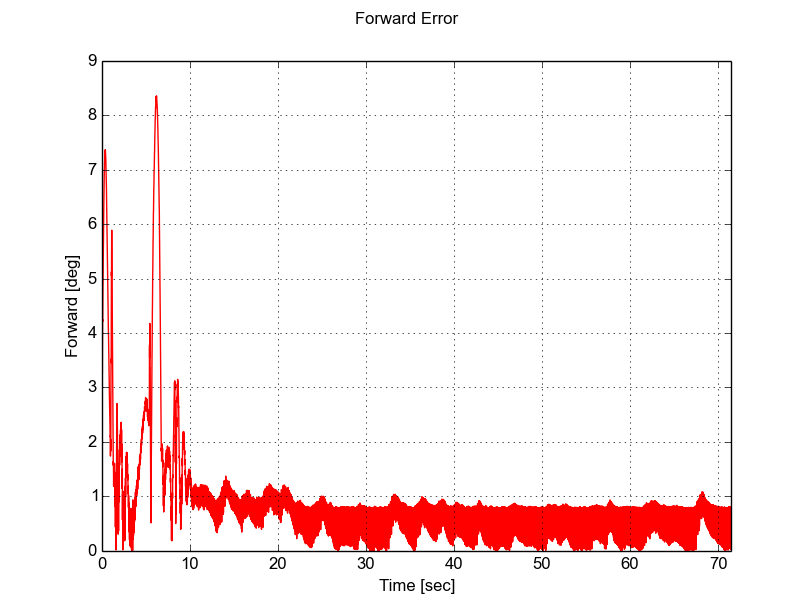
\includegraphics[width=\textwidth]{circle_fwd_error}
    \caption{Forward error}
    \label{fig:circle_fwd_error}
  \end{subfigure}
  ~ %add desired spacing between images, e. g. ~, \quad, \qquad, \hfill etc.
    %(or a blank line to force the subfigure onto a new line)
  \caption{Circle trajectory performance.}
  \label{fig:circle_performance}
\end{figure}

\pagebreak
\subsection{Lissajous Trajectory}
The second trajectory was based on a Lissajous curve, defined by:
\begin{align}
  x_d(t) &=
  \begin{bmatrix}
    A \cos(\omega_a t) \\
    B \sin(\omega_b t) \\
    C \sin(\omega_c t) + Z
  \end{bmatrix}
\end{align}
with $A = B = 6$ m, $C = 4$ m, $Z = 5$ m, $T_a = 2 \pi/ \omega_a = 8.33$ sec,
$T_b = 12.5$ sec, and $T_c = 25$ sec.

Again, the forward vector was set to $f_d(t) = \frac{v_d(t)}{||v_d(t)||}$, where the
velocity vector $v_d(t) = \dot{x}(t)$ is given by
\begin{align}
  v_d(t) &=
  \begin{bmatrix}
    -A \omega_a \sin(\omega_a t) \\
    B \omega_b \cos(\omega_b t) \\
    C \omega_c \cos(\omega_c t)
  \end{bmatrix}.
\end{align}

Figure \ref{fig:lissajous_performance} show the tracking
performance for the controller. As once can see, the controller successfuly
tracks this more aggressive trajectory, although the steady state errors are
more significant than for the simpler cicular trajectory. The RMSE for each
position and orientation component is shown in Table \ref{table:metrics}.

\begin{figure}[h]
  \centering
  \begin{subfigure}[b]{0.45\textwidth}
    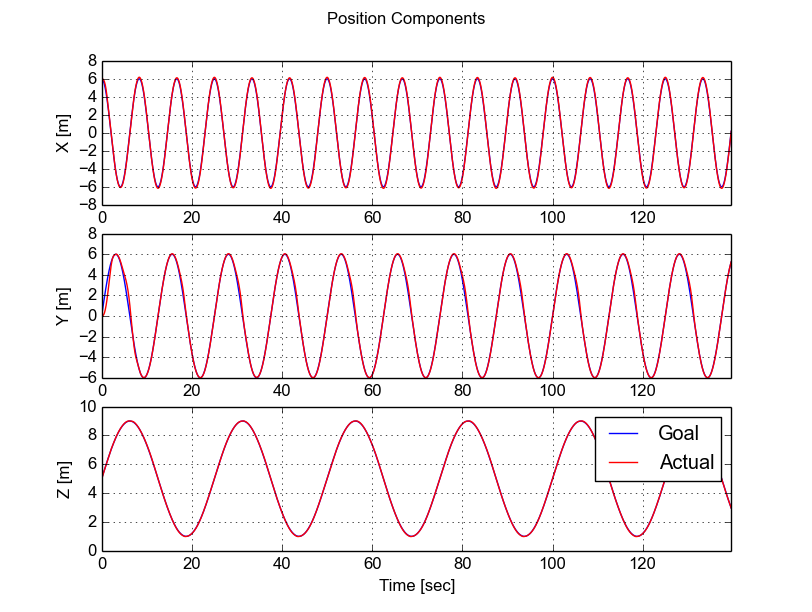
\includegraphics[width=\textwidth]{lissajous_position}
    \caption{Position}
    \label{fig:lissajous_position}
  \end{subfigure}%
  ~ %add desired spacing between images, e. g. ~, \quad, \qquad, \hfill etc.
    %(or a blank line to force the subfigure onto a new line)
  \begin{subfigure}[b]{0.45\textwidth}
    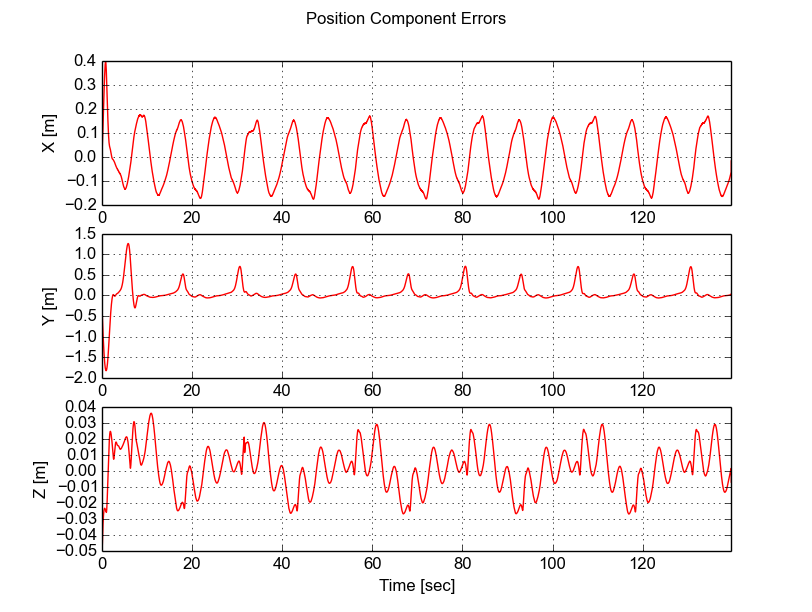
\includegraphics[width=\textwidth]{lissajous_position_errors}
    \caption{Position errors}
    \label{fig:lissajous_position_errors}
  \end{subfigure}

  \begin{subfigure}[b]{0.45\textwidth}
    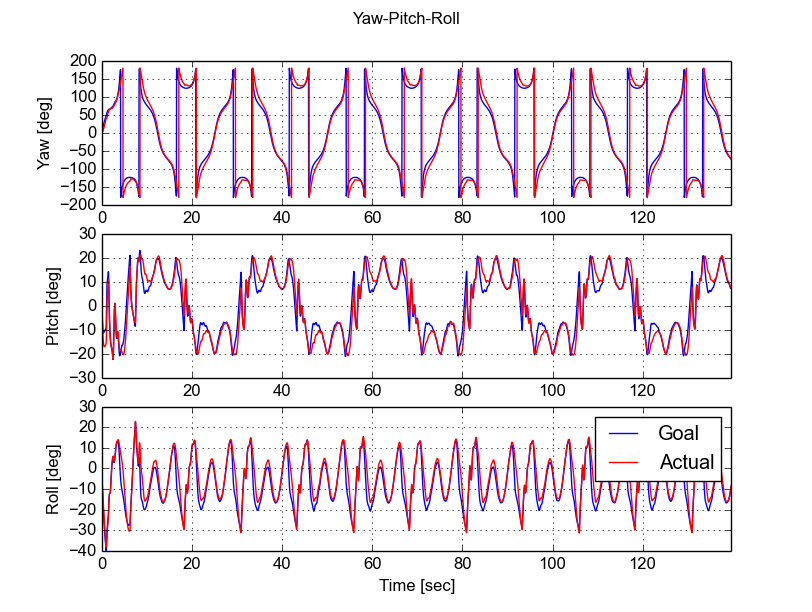
\includegraphics[width=\textwidth]{lissajous_yaw_pitch_roll}
    \caption{Yaw, pitch, and roll}
    \label{fig:lissajous_yaw_pitch_roll}
  \end{subfigure}%
  ~ %add desired spacing between images, e. g. ~, \quad, \qquad, \hfill etc.
    %(or a blank line to force the subfigure onto a new line)
  \begin{subfigure}[b]{0.45\textwidth}
    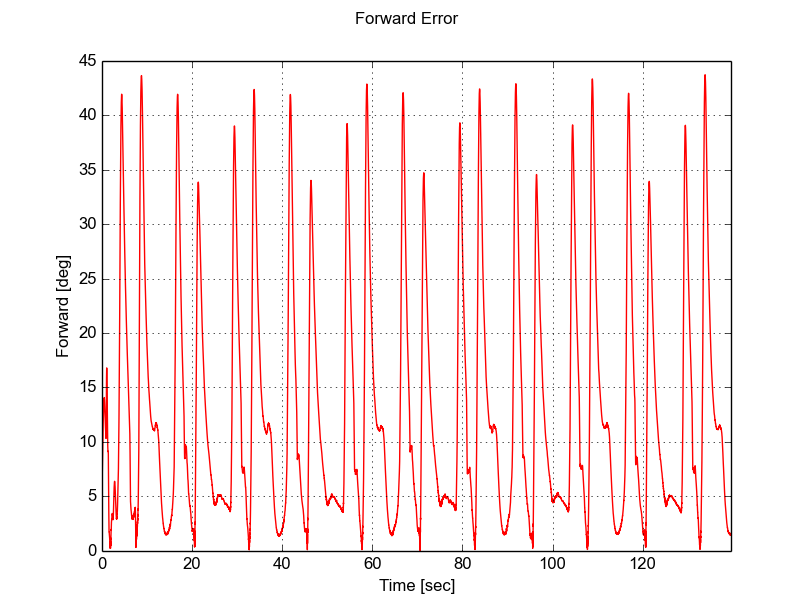
\includegraphics[width=\textwidth]{lissajous_fwd_error}
    \caption{Forward error}
    \label{fig:lissajous_fwd_error}
  \end{subfigure}
  ~ %add desired spacing between images, e. g. ~, \quad, \qquad, \hfill etc.
    %(or a blank line to force the subfigure onto a new line)
  \caption{Lissajous trajectory performance.}
  \label{fig:lissajous_performance}
\end{figure}

\pagebreak
\begin{table}[b]
\centering
\begin{tabular}[h]{|c|c|c|c|c|}
  \hline
   & x [cm] & y [cm] & z [cm] & f [deg] \\
  \hline
  Circle & 9.46 & 64.9 & 0.95 & 1.38 \\
  \hline
  Lissajous & 11.4 & 25.9 & 1.39 & 17.1 \\
  \hline
\end{tabular}
\caption{RMSE tracking performance for two simulated trajectories.}
\label{table:metrics}
\end{table}

\section{Conclusion and Future Directions}
This project successfully implemented a modified version of a novel, nonlinear
controller for aggressive quadrotor flight based on \cite{lee2010geometric}
using the \texttt{hector\_quadrotor} stack and
validated its performance on two trajectories of varying complexity.
Performance metrics show that the controller can easily track simple flight
maneuvers outside of the hover state and can adequately track complex trajectories
with significant angular accelerations.

Future work to consider would be to remove the inner PID control loop and
control the thrust $f$ and torque $M$ directly, which should allow tracking
more extreme manuevers. One might also consider the automatic generation of
dynamically feasible paths through minimum snap optimzation as in
\cite{mellinger2011minimum} or \cite{richter2013polynomial}. Finally, it would be
interesting to test the controller outside of simulation using an actual quadrotor.

%----------------------------------------------------------------------------------------
% Bibliography
%----------------------------------------------------------------------------------------
\clearpage
\bibliography{references}{}
\bibliographystyle{plain}

\end{document}
